\chapter{Identification des demandes}
%\chapter{Extraction des demandes et résultats correspondants}
\label{chap:quanta}

\textit{\small \textbf{Résumé.} Ce chapitre aborde le problème d'identification automatique, dans une décision, des éléments structurants les demandes formulées. L'identification manuelle réalisée à travers la lecture exige beaucoup d'effort à cause de la complexité du contenu dans lequel les demandes sont mélangées à d'autres informations (des demandes de nature différente, des arguments, des faits, etc.). L'automatisation de cette tâche métier vise à aider les experts à rapidement comprendre les réclamations des parties et les réponses correspondantes des juges. Une demande est abstraite par cinq attributs : la norme qui la fonde, son objet, l'interprétation du résultat ($s_r$), le quantum demandé ($q_d$), et celui obtenu ($q_r$). La norme et l'objet forment ensemble la catégorie de la demande. L'annotation manuelle des données d'évaluation suit un protocole que nous avons précisément défini avec l'expert du projet. Ce protocole recommande des cycles d'annotation consistant chacun à constituer un ensemble de décisions et à y identifier toutes les demandes d'une seule catégorie donnée car il serait difficile d'annoter simultanément des données pour toutes les catégories qui sont très nombreuses. L'approche proposée extrait à chaque application les demandes d'une seule catégorie et est formulée en trois tâches. La présence de la catégorie est déterminée par classification de la décision. Ensuite, les quanta et le sens du résultat sont identifiés à proximité de termes appris de la catégorie dans les sections adéquates identifiées à l'aide d'un modèle à base de CRF comme décrit au chapitre \ref{chap:structuration}. Enfin, les demandes sont formées en mettant en correspondance les éléments précédemment déterminés. Réalisées par validation croisées, nos expérimentations comparent une douzaine de méthodes statistiques d'extraction de termes-clés et quatre algorithmes de classification pour l'extraction de 6 catégories prédéfinies de demandes. Les résultats montrent que la détection de catégorie est facile quelque soit l'algorithme utilisé ($F_1$-mesure comprise entre 98.8 \% et 100 \%). Il résulte aussi que l'extraction des demandes nécessite de sélectionner la méthode d'extraction de terminologie la mieux adaptée à la catégorie. Cette sélection préalable permet d'observer, sur les données de test, des $F_1$-mesures comprises entre 33.09 \% et 71.43 \% pour les champs $q_d$, $q_r$, et $s_r$, et entre 28.65 \% et 58.99 \% pour les triplets $(q_d,s_r, q_r)$.}

\section{Introduction}
\label{sec:quanta:introduction}

%\textcolor{red}{Introduire, chaque chapitre, de manière explicite par la contribution, discuter l'impacte de chaque méthode explorée, contribution sur la constitution des datasets, accompagnement des experts. dans un encadré}

Au c\oe{}ur de l'analyse des décisions de justice se trouve le concept de demande. Il s'agit d'une réclamation ou requête effectuée par une ou plusieurs parties aux juges. Une partie peut demander des dommages-intérêts en réparation d'un préjudice subi ou à l'issu d'un divorce, des indemnités auxquelles elle pense avoir droit, ou encore une étude d'expert, etc. Les demandes sont fondamentales car l'argumentation au cours d'une affaire a deux buts : faire accepter ses demandes, et faire rejeter celles de la partie adverse. L'extraction des demandes et des résultats correspondants, dans un corpus, permet ainsi de récolter des données informant de la manière dont sont jugés des types de demandes d'intérêt. Les informations qui nous intéressent sont la catégorie de la demande, le quantum (montant) demandé, le sens du résultat (par ex. la demande a-t-elle été acceptée ou rejetée ?), et le quantum obtenu (décidé par les juges). Pour pouvoir extraire les demandes et les résultats, il est nécessaire de comprendre comment ceux-ci sont exprimés et co-référencés dans les décisions jurisprudentielles. Leur énoncé peut comporter des expressions plus ou moins complexes, dont souvent des références à des jugements antérieurs, des agrégations ou des restrictions (\figureref{fig:quanta:expr-dmd-rst}).

\begin{figure}[ht]
	\footnotesize
\begin{center}
	\begin{subfigure}[t]{0.95\textwidth}
		\fbox{\parbox{\textwidth}{Jennifer M., Catherine M. et Sandra M. ... demandent à la Cour de :
				
				- les recevoir régulièrement appelantes incidentes du \textcolor{blue}{jugement du 23/05/2014} ;
				
				- infirmer \textcolor{blue}{le dit jugement} en \textcolor{brown}{toutes ses dispositions} ; ...
				
				Statuant à nouveau ...
				
				- \textcolor{brown}{les condamner au paiement d'une somme de 3 000,00 \euro{} pour procédure abusive et aux entiers dépens} ; }}
		\caption{Exemples d'énoncés de demandes}\label{fig:quanta:expr-dmd}
	\end{subfigure} 
	
	
	\begin{subfigure}[t]{0.95\textwidth}
		\fbox{\parbox{\textwidth}{La cour, ... 
				
				CONFIRME \textcolor{blue}{le jugement entreprise} en \textcolor{brown}{toutes ses dispositions}.
				
				Y ajoutant
				
				\textcolor{gray}{CONSTATE que Amélanie Gitane P. épouse M. est défaillante à rapporter la preuve
					d'une occupation trentenaire lui permettant d'invoquer la prescription
					acquisitive de la parcelle BH 377 située [...].}
				
				\textcolor{gray}{DEBOUTE Amélanie Gitane P. épouse M. de sa demande en dommages et intérêts.}
				
				\textcolor{gray}{CONDAMNE Amélanie Gitane P. épouse M. aux dépens d'appel.}
				
				\textcolor{gray}{DIT n'y avoir lieu à l'application de l'article 700 du Code de Procédure Civile.}
		}}
		\caption{Exemple d'énoncés de résultats}\label{fig:quanta:expr-rst}
	\end{subfigure}
\end{center}

\textit{\textbf{Source:} extraits de la décision 14/01082 de la cour d'appel de Saint-Denis (Réunion).}

\textit{\textbf{Légende:} énoncés simples en \textcolor{gray}{gris}, références en \textcolor{blue}{bleu}, et agrégations en \textcolor{brown}{marron}.}
	\caption{Illustrations de la complexité des énoncés de demandes et de résultats.}\label{fig:quanta:expr-dmd-rst}
\end{figure}


\subsection{Données cibles à extraire}

\subsubsection{Catégorie de demande}

Une catégorie $c$ de demande regroupe les prétentions qui sont de même nature par le fait qu'elles partagent deux aspects : l'objet demandé (par ex. dommages-intérêts, amende civile, déclaration de créance) et le fondement c'est-à-dire les règles ou normes ou principes juridiques qui fondent la demande (par ex. article 700 du code de procédure civile). Des noms particuliers sont utilisés pour identifier les catégories (Tableau \ref{tab:quanta:exemple-categorie}).

\begin{table}[!htb]
\small
\begin{tabular}{|c|p{0.35\textwidth}|p{0.15\textwidth}|p{0.3\textwidth}|}
\hline
\textbf{Label} & \textbf{Nom} & \textbf{Objet} & \textbf{Fondement} \\ \hline
\textit{acpa} & amende civile pour abus de procédure & amende civile & Articles 32-1 code de procédure civile + 559 code de procédure civile \\ \hline
\textit{concdel} & dommages-intérêts pour concurrence déloyale & dommages-intérêts & Article 1382 du code civil \\ \hline
\textit{danais} & dommages-intérêts pour abus de procédure & dommages-intérêts & Articles 32-1 code de procédure civile + 1382 code de procédure civile \\ \hline
\textit{dcppc} & déclaration de créance au passif de la procédure collective & déclaration de créance & L622-24 code de commerce \\ \hline
\textit{doris} & dommages-intérêts pour trouble de voisinage & dommages-intérêts & principe de responsabilité pour trouble anormal de voisinage \\ \hline
\textit{styx} & frais irrépétibles & dommages-intérêts & Article 700 du code de procédure civile \\ \hline
\end{tabular}
\textit{Les labels ont été définis dans le cadre du projet, et par conséquent, ils n'existent pas dans le langage juridique.}
\caption{Exemples de catégories de demandes.}\label{tab:quanta:exemple-categorie}
\end{table}

\subsubsection{Sens du résultat}

Le sens du résultat est l'interprétation de la décision des juges sur une demande. Nous le notons $s_r$. En général, le sens peut être positif si la demande a été acceptée, et négatif si elle a été rejetée. Il arrive aussi que le résultat soit reporté à un jugement futur ; il s'agit dans ce cas d'un sursis à statuer. 

\subsubsection{Quantum demandé}

Le quantum demandé quantifie l'objet de la demande. Nous le notons $q_d$. Par exemple, dans l'exemple de la Figure \ref{fig:quanta:expr-dmd}, "3000 \euro{}" est le quantum demandé au titre des dommages-intérêts pour procédure abusive. Bien que cette étude ne porte que sur des sommes d'argent, le quantum peut être d'une autre nature comme par exemple une période dans le temps (garde d'enfant, ou emprisonnement, etc.). Toutes les catégories demandes n'ont pas de quantum (par ex. une demande de divorce) et seul le sens du résultat sera la donnée à extraire dans ce cas.


\subsubsection{Quantum obtenu ou résultat}

Le quantum obtenu quantifie le résultat ou la décision des juges. Nous le notons $q_r$. Il ne peut qu'être inférieur ou égal au quantum demandé. Si la demande est rejetée, 
$q_r$ est nul même si cela n'est pas explicitement mentionné dans le document. A noter qu'il doit être de la même nature que le quantum demandé (somme d'argent ou durée).


\subsection{Expression, défis et indicateurs d'extraction}

Les demandes sont en général décrites à la fin de la section d'exposé des faits, procédures, moyens et prétentions des parties (section Litige cf. \ref{sec:structuration:sectionnement-en-4} et \ref{appendix:exemple-decision}). Elles rentrent donc dans les "moyens et prétentions des parties" qui regroupent les demandes et les arguments des parties. Quant aux résultats, ils sont décrits dans la section Dispositif et dans la section Motifs (raisonnement des juges). Les demandes sont exprimées dans différents paragraphes qui correspondent soit à une partie, soit à un groupe de parties partageant les mêmes demandes (par ex. des époux). Les paragraphes sont parfois organisés en liste dont chaque élément exprime une ou plusieurs demandes, ou fait référence à un jugement antérieur. Les résultats ont aussi la forme de liste dans la section Dispositif. Par contre, dans les motifs de la décision, les raisonnements sont organisés en paragraphes, et ordonnés catégorie après catégorie. Le résultat est donné à la fin du groupe de paragraphes associé à la catégorie.


 Cette pseudo-structure n'est pas standard et impose de nombreux défis à relever. En effet, une décision jurisprudentielle porte sur plusieurs demandes de catégories différentes ou similaires. Il est important de faire correspondre un quantum demandé extrait au sens et quantum du résultat qui font référence à la même demande. La séparation des demandes et des résultats rend difficile cette mise en correspondance. Ce problème peut aussi être causé par la redondance des quanta ; par exemple, les résultats exprimés dans les Motifs sont résumés dans le Dispositif. D'autre part, les références aux jugements antérieurs exigent de résoudre des références aux résultats de jugements antérieurs qui sont, généralement, rappelés dans le même document. Notons aussi que les difficultés liées aux agrégations (par ex. "\textit{infirmer ... en toutes ces dispositions}") et aux restrictions/sélections (par ex. "\textit{infirme le jugement ... sauf en ce qu'il a condamné M. A. ...}") méritent d'être résolues. Par ailleurs, les catégories de demandes sont nombreuses\footnote{plus de 500 selon la nomenclature des affaires civiles NAC+.} mais ne sont pas toutes présentes à la fois dans les décisions. Tous ces aspects rendent difficile l'annotation manuelle des données de référence et la modélisation d'une approche d'extraction adéquate. Nous avons cependant identifié des indicateurs qui pourraient être utiles.

On pourrait au préalable annoter les candidats potentiels de quanta. Nous nous sommes intéressés aux demandes dont les quanta sont des sommes d'argent. Les mentions de somme d'argent sont généralement de la forme \og \texttt{[valeur] [monnaie]} \fg{} (par ex. \texttt{3000 \euro}, \texttt{15 503 676 francs}, \texttt{un euro}, \texttt{339.000 XPF}). Des centimes apparaissent parfois (par ex. \texttt{dix huit euros et soixante quatorze centimes}, \texttt{26'977 \euro{} 19}). Ainsi, il est possible d'annoter les sommes d'argent à l'aide d'une expression régulière. Même s'il est difficile de reconnaître des sommes d'argent écrites en lettre, il faut remarquer que l'équivalent en chiffre est généralement mentionné tout près (par ex. \texttt{neuf mille cinq cent soixante six euros et quatre vingt sept centimes (9566,87 \euro{})}). 

La terminologie utilisée est aussi un bon indicateur pour reconnaître des demandes et des résultats. En effet, le vocabulaire utilisé est très souvent propre aux catégories de demandes. Par exemple le dernier élément de la Figure \ref{fig:quanta:expr-dmd} comprend le terme "\textit{pour procédure abusive}" qui est près d'une somme d'argent (\textit{3000 \euro{}}) ; il est donc probable que ce type de terme assez particulier soit un bon indicateur de la position des quanta. Par ailleurs, des verbes particuliers sont utilisés pour exprimer les demandes et résultats : infirmer, confirmer, constater, débouter, dire ... %Comme autres formes récurrentes, on pourrait citer l'ordre des demandes (resp. résultats). Généralement, on a les constats, les références aux jugements antérieurs, les demandes principales (?) et secondaires (?).




% Dans la section suivante, nous discutons de l'analogie de l'extraction des demandes avec d'autres problématiques d'extraction d'information. 


\subsection{Formulation du problème}
\label{sec:quanta:formulation}

Nous avons tenu compte de deux principaux aspects du problème :
\begin{enumerate}
	\item Une décision comprend plusieurs demandes de catégories similaires ou différentes;
	\item Il existe un grand nombre de catégories (500+) ; ce qui rend difficile l'annotation d'exemples de référence pour couvrir toutes ces catégories.
\end{enumerate}

 L'idée est de pouvoir ajouter progressivement de nouvelles catégories. Nous avons par conséquent opté pour une extraction par catégorie. Cette stratégie permet par ailleurs d'ajouter facilement de nouvelles catégories sans avoir à redéfinir les catégories déjà entraînées. Une exécution du système d'extraction permet ainsi d'extraire les demandes d'une seule catégorie. Le problème est décomposé en deux tâches :
\begin{description}
	\item[Tâche 1 :] Détecter les catégories présentes dans le document pour appliquer l'extraction uniquement à ces catégories;
	\item[Tâche 2 :] Pour chaque catégorie $c$ identifiée, extraire les demandes :
	\begin{enumerate}
		\item identification des valeurs d'attributs : quanta demandés ($q_d$), quanta obtenus ($q_r$), et sens du résultat ($s_r$);
		\item mise en correspondance des attributs pour former les triplets ($q_d, s_r, q_r$) correspondants aux paires demande-résultat.
	\end{enumerate}
\end{description}

%L'annotation des candidats de quanta, les sommes d'argent dans notre cas, doit être réalisée préalablement à la seconde tâche.
 
\section{Travaux connexes}
\label{sec:quanta:biblio}
Chacune des tâches précédentes se rapproche d'une tâche couramment traitée en fouille de textes. En effet, la détection de catégories dans les décisions peut être modélisée comme un problème de classification de documents. La tâche d'extraction se rapproche plus quant à elle des problématiques comme l'extraction d'évènements, le remplissage de champs, ou encore l'extraction de relations et la résolution de référencement.

\subsection{Extraction d'éléments structurés}% avec des problématiques d'extraction d'information}

Les demandes ressemblent aux structures telles que les relations ou les évènements. En effet, les champs définis par la compétition d'Extraction Automatique de Contenus ACE (\textit{Automatic Content Extraction}), dans \citet{ace2005relation}, pour les relations et \citet{ace2005event} pour les évènements, se rapprochent de ceux visés lors de l'extraction des demandes comme l'illustre le  \tableref{tab:quanta:analogie-relation-evt}. Plus précisément, une catégorie de demandes correspond à un type d'évènement ou de relation entre deux entités. Les arguments qui participent à l'évènement \og demande \fg{} ou à la relation \og demande-résultat \fg{} sont le quantum demandé et le quantum résultat. Le sens du résultat représente la classe de la structure \og demande \fg{}.

\begin{table}[!htb]
	\footnotesize
	\begin{tabular}{|p{0.15\textwidth}|p{0.21\textwidth}|p{0.21\textwidth}|p{0.30\textwidth}|}
		\hline		%\textbf{Champs} 
		 & \textbf{Relation \citep{ace2005relation}} & \textbf{Événement \citep{ace2005event}} & \textbf{Analogie chez les demandes} \\ \hline
		\textbf{Type} & Org-Aff.Student-Alum & Die & Catégorie="Dommages-intérêts pour procédure abusive" \\ \hline
		\textbf{Passage} (\textit{extend}) & \textit{Card graduated from the University of South Carolina} & "Il est mort hier d'une insuffisance rénale." & (\textit{Figure \ref{fig:quanta:expr-dmd-rst}}) \\ \hline
		\textbf{Déclencheur (\textit{trigger})} & - & "mort" & "procédure abusive"\\ \hline
		\textbf{Participants ou Arguments (\textit{arguments})} & Arg1="Card" \linebreak Arg2="the University of South
		Carolina"& Victim-Arg="il" \linebreak Time-Arg="hier" & Quantum-demandé="3000\euro{}"\linebreak Quantum-obtenu="0 \euro{}"\ \\ \hline
		\textbf{Classes (\textit{attributes, classes})} & Asserted & Polarity=POSITIVE, Tense=PAST & Sens-résultat="Rejeté" \\ \hline
	\end{tabular}
	\caption{Exemples d'analogie entre relations, évènements et demandes.} \label{tab:quanta:analogie-relation-evt}
\end{table}

\subsection{Approches d'extraction d'éléments structurés}
\label{quanta:related-approaches}
L'extraction d'éléments structurés repose généralement sur une approche modulaire du problème qui le décompose en tâches plus simples. D'une part, on dispose de l'identification des déclencheurs\footnote{Terme-clés indiquant la présence d'un évènement \citep{ace2005event}.} et des arguments. D'autre part, une mise en correspondance relie les arguments et déclencheurs qui participent à la même relation ou au même évènement. Les classes peuvent être déterminées par classification du passage associé. Cette décomposition a permis à de nombreuses méthodes de voir le jour. 

L'approche traditionnelle consiste en une chaîne de traitements enchaînant des modules adaptés à une tâche simple. La sortie d'une étape est l'entrée de la suivante. C'est ainsi que \citet{ahn2006stages} définit un enchaînement de modèles de classification (k-plus-proches-voisins \citep{cover1967knn} vs. classificateur d'entropie maximum \citep{nigam1999maxent}), pour extraire des champs d'évènements dans le corpus d'ACE\citet{ace2005event}. Bien que les différents modules soient plus faciles à développer, ce type d'architecture souffre de la propagation d'erreurs d'une étape à la suivante, ainsi que de la non exploitation de l'interdépendance entre les tâches. Par conséquent, l'inférence jointe des champs est préconisée. Celle-ci peut-être réalisée par une modélisation graphique probabiliste ou neuronale. Par exemple, pour l'extraction d'évènements, \citet{yang2016jointEntityEvt} estiment la probabilité conditionnelle jointe du type d'entité $t_i$, les rôles des arguments $r_{i\cdot}$ et les types d'entités qui remplissent ces rôles $a.$ : $p_\theta(t_i,r_{i\cdot},a. \vert i, N_i, x)$, $i$ étant un déclencheur candidat, $N_i$ l'ensemble des entités candidates qui sont de potentiels arguments pour $i$, et $x$ est le document. Cette approche obtient 50.6\% de $F_1$-mesure moyenne pour la détection des valeurs d'arguments et 48.4\% pour leur classification dans leur rôle respectif. Par ailleurs, \citet{nguyen2016jointtrgarg} illustrent l'utilisation des réseaux de neurones profonds avec une couche pour la prédiction du déclencheur, une autre pour le rôle des arguments, et la dernière encode la dépendance entre les labels de déclencheurs et les rôles d'arguments. Cette approche obtient 62.8\% de $F_1$-mesure moyenne pour la détection des valeurs d'arguments et 55.4\% pour leur classification dans leur rôle respectif. %\textcolor{red}{[PERFORMANCE DE LEUR METHODE]} 

L'annotation du corpus de l'ACE est un marquage des champs dans le texte, et par conséquent, la position ou l'occurrence des champs est indiquée (\og annotation au niveau du segment de mots \fg{}). Comme dans notre cas, les données peuvent être annotées dans un tableau, hors des textes d'où elles sont issues. Il est donc nécessaire de retrouver leur position sans supervision. \citet{palm2017e2e-dnn} proposent dans cette logique une architecture de réseaux de neurones point-à-point qu'ils ont expérimentés sur des corpus de requêtes de recherche de restaurant et films \citep{liu2013mitmovierestaurant} ou de réservation de billets d'avion \citep{price1990atis}. Ils se sont intéressés au problème de remplissage de champs en apprenant la correspondance entre les textes et les valeurs de sorties. Leur modèle est basé sur les réseaux de pointeurs \citep{vinyals2015pointernetworks} qui sont des modèles séquence-à-séquence avec attention, dans lesquels la sortie est une position de la séquence d'entrée. Le modèle proposé consiste en un encodeur de la phrase et des contextes, plusieurs décodeurs (un pour chaque champ). L'application de cette architecture à l'extraction des demandes serait confrontée à deux obstacles majeurs auxquels il faut répondre au préalable. Premièrement, les décisions judiciaires ont des contenus de plusieurs centaines à plusieurs milliers de lignes contrairement aux requêtes manipulées par \citet{palm2017e2e-dnn} dont la plus longue ne comprend que quelques dizaines de mots. La complexité des architectures neuronales de TALN augmente rapidement en espace et en temps avec la longueur des documents manipulés. Deuxièmement, nous disposons de très peu de données annotées ; entre 23 et 198 documents annotés dans notre cas contre plusieurs milliers pour les expérimentations de \citet{palm2017e2e-dnn}.

L'avantage de l'utilisation des réseaux de neurones vient de leur capacité à apprendre automatiquement des caractéristiques pertinentes contrairement aux modèles probabilistes qui exigent très souvent une ingénierie manuelle des caractéristiques. Par contre, il est beaucoup plus facile d'utiliser les modèles probabilistes sur des corpus de faible taille et de longs textes comme c'est le cas pour le problème d'identification des demandes judiciaires.


\subsection{Extraction de la terminologie d'un domaine}
\label{sec:quanta:extract-terminologie-domaine}
L'identification des attributs peut être facilitée grâce à leur proximité avec des termes-clés caractéristiques des catégories de demandes au même titre que les \og déclencheurs \fg{} aident à identifier les évènements.
Ne disposant pas au préalable de la liste des termes pertinents pour l'extraction des demandes, il est possible de les apprendre. Il existe à cet effet plusieurs métriques statistiques de pondération de termes généralement employées en recherche d'information et en classification de texte comme méthodes de sélection de caractéristiques. Ces métriques sont qualifiées de poids globaux car calculées à partir des occurrences dans un corpus, à la différence des poids locaux (Tableau \ref{tab:sensresultat:metriq_locales}) calculés à partir des occurrences dans un document. Quelques métriques sont formulées ici en utilisant les notations du Tableau \ref{tab:quanta:notations_metriques} définies pour une base d'apprentissage.


%Les approches d'extraction de terminologie peuvent être organisés dans les principaux groupes suivants \citet{gomez2004overviewontologielearning,lossio2014biotexcvalue}: 
%\begin{enumerate}
%	\item les approches à base de techniques linguistiques qui consistent à reconnaitre les termes-clés à l'aide de motifs linguistiques \citep{gaizauskas2000linguistictermrecognition}. comme des expressions régulières de groupes grammaticaux à l'instar de la combinaison $(Adj\vert Nom)^+Nom$.
%	\item les approches à base de techniques statistiques qui permettent d'affecter des scores aux termes d'un corpus et par conséquent de les ranger par ordre de pertinence. On a pour exemple la métrique IDF (\textit{Inverse Document Frequency}) de \citet{sparck1972idf}. 
%	\item les approches à base d'algorithmes d'apprentissage automatique à l'instar des architectures d'apprentissage profond entrainées par \citet{gharbieh2017deeptermlearning} pour apprendre des expressions à mots multiples.
%	\item Les approches hybrides combinent différentes méthodes par exemple la méthode C-value \citep{frantzi2000CValueNCValue} réalise une sélection préalable de candidats par des filtres linguistiques, puis pondère les différents candidats pour en distinguer les plus pertinents.
%\end{enumerate}
%\subsubsection{Méthodes statistiques}
% LISTES POUR CHAQUE CATÉGORIE
\begin{table}[!htb]
	\centering
	\begin{tabular}{lp{0.8\textwidth}}
		\hline\noalign{\smallskip}
		Notation & Description \\
		\noalign{\smallskip}
		\hline
$t$ & un terme \\
$d$& un document \\
$\vert t \vert$ & longueur de $t$ (nombre de mots) \\
$c$ & la catégorie (domaine ciblé) \\
$\overline{c}$ & la classe complémentaire ou négative \\
$D$& ensemble global des documents de taille $N = \vert D \vert$ \\
$D_{c}$& ensemble des documents de $c$ de taille $\vert D_{c} \vert$ \\% = $N^+$\\
$D_{\overline{c}}$& ensemble des documents de $\overline{c}$ de taille $\vert D_{\overline{c}} \vert$\\% = $N^-$\\
$N$& nombre total de documents\\
$N_{t}$& nombre de documents contenant $t$\\
$N_{\overline{t}}$& nombre de documents ne contenant pas $t$\\
$N_{t,c}$ & nombre de documents de $c$ contenant $t$\\
$N_{\overline{t},c}$ & nombre de documents de $c$ ne contenant pas $t$\\% = $b$\\
$N_{t,\overline{c}}$ & nombre de documents de $\overline{c}$ contenant $t$\\% = $c$\\
$N_{\overline{t},\overline{c}}$ & nombre de documents de $\overline{c}$ ne contenant pas $t$\\% = $d$\\
%$\vert D \vert$ & nombre total de documents ($\vert D \vert = \vert D_{c} \vert + \vert D_{\overline{c}} \vert$)\\
%$DF_c$ & proportion de documents du corpus appartenant à $c$ (probabilité qu'un texte pris au hasard soit de la classe $c$ )\\
%$DF_t$& proportion de documents du corpus contenant $t$ (\textit{Document Frequency})\\
$DF_{t \vert c}$ & proportion de documents contenant $t$ dans le corpus de $c$ ($DF_{t \vert c} = \frac{N_{t,c}}{\vert D_c \vert}$) \\
$DF_{c \vert t}$ & proportion de documents appartenant à $c$ dans l'ensemble de ceux qui contiennent $t$ \\
\hline
\end{tabular}
\caption{Notation utilisée pour formuler les métriques} \label{tab:quanta:notations_metriques}
\end{table}

% Lorsque la fonction n'utilise que le corpus représentatif du domaine d'intérêt, elle mesure ainsi le degré d'importance du terme dans le langage d'un domaine particulier ou une classe particulière de documents. Par exemple, la fonction \og fréquence de document \fg{} (\textit{DF - Document Frequency}) mesure l'importance d'un terme en lui affectant la proportion de documents qui le contiennent dans un corpus global considéré. De telles fonctions sont qualifiées de non-supervisées contrairement à celles qui se calculent entre différents corpus et par conséquent utilisent les labels des données d'entraînement \citep{lan2009termweighting, wu2017balancingtermweight}. Ces dernières mesurent l'importance du terme dans la discrimination (ou la différence) entre le domaine d'intérêt et les autres corpus. Un exemple simple s'obtient en faisant la différence de \og fréquence de document \fg{} d'un terme entre un corpus $c$ et sont complémentaire $\overline{c}$. 

\subsubsection{Métriques non-supervisées}
Les métriques non-supervisées affectent un score à un terme en rapport avec l'importance de ce dernier dans le corpus global $D$. Parmi ces métriques, on retrouve par exemple la fréquence inverse de document (\textit{inverse document frequency}) $idf$ \citep{sparck1972idf} et ses variantes $pidf$ \citep{wu1981pidf} et $bidf$ \citep{jones2000bm25idf} accordent plus d'importance aux termes rares. Elles considèrent en fait qu'un terme rare est plus efficace pour la distinction entre des documents. Par conséquent, elles sont efficaces en recherche d'information mais moins indiquées en classification de textes où le but est plutôt de séparer des catégories \citep{wu2017balancingtermweight}. Elles se formulent comme suit :
\[idf(t) = \log_2\left(\frac{N}{N_t}\right), pidf(t) = \log_2\left(\frac{N}{N_t} - 1\right), bidf(t) = \log_2\left(\frac{N_{\overline{t}} + 0.5}{N_t + 0.5}\right)\]

Il est possible de prendre explicitement en compte le fait que les termes peuvent comprendre plusieurs mots (n-grammes) et avoir des tailles différentes (nombre de mots). La $\text{C-value}$ \citep{frantzi2000CValueNCValue}, par exemple, distingue la fréquence du terme et de ses sous-termes (termes imbriqués) par la formule : % t \mbox{ n'est imbriqué dans aucun terme candidat}
\[\text{C-value}(t) = \begin{cases} \log_2(\vert t \vert) \cdot (N_t - \frac{1}{\vert T_t \vert} \cdot \sum\limits_{b \in T_t} N_b), & \mbox{si } t \mbox{ est imbriqué} \\ \log_2(\vert t \vert) \cdot N_t, & \mbox{sinon,} \end{cases}\]
$T_t$ étant l'ensemble des termes candidats qui contiennent $t$.


\subsubsection{Métriques supervisées}
\label{sec:quanta:poids-globaux-superv}
Les métriques supervisées mesurent l'information contenue dans les labels des documents de la base d'apprentissage. Pour un terme $t$, elles expriment généralement la différence de proportion qui existe entre les occurrences de $t$ dans $D_c$ et ses occurrences dans $D_{\overline{c}}$. Elles sont ainsi mieux adaptées à la distinction entre catégories. Parmi les nombreuses métriques existantes, nous avons expérimenté les suivantes : 
\begin{description}
	\item[La différence de fréquence] $\Delta_{DF}$ consiste simplement à calculer la différence entre les proportions de documents contenant $t$ respectivement dans $c$ et $\overline{c}$ :
	\[\Delta_{DF}(t,c) = DF_{t \vert c} - DF_{t \vert \overline{c}}\]
	\item[Le gain d'information] $ig$ \citep{yang1997IGandIMandCHIandTS} estime la quantité d'information apportée par la présence ou l'absence d'un terme $t$ sur l'appartenance d'un document à une classe $c$ :
	\begin{equation*} % A VERIFIER
	ig(t, c) = \splitdfrac{\frac{N_{t,c}}{N} \log_2 \left(\frac{N_{t,c}N}{N_{t}}\right)
		 + \frac{N_{\overline{t},c}}{N} \log_2 \left(\frac{N_{\overline{t},c}N}{N_{\overline{t}}\vert D_c \vert}\right)}
	{+ \frac{N_{t,\overline{c}}}{N} \log_2 \left(\frac{N_{t,\overline{c}}N}{N_{t}\vert D_{\overline{c}}\vert}\right)
	+ \frac{N_{\overline{t},\overline{c}}}{N} \log_2 \left(\frac{N_{\overline{t},\overline{c}}N}{N_{\overline{t}}\vert D_c \vert}\right)}
	\end{equation*}
	\item[La fréquence de pertinence] $rf$ \citep{lan2009rf} a comme intuition de considérer que plus la fréquence d'un terme $t$ est élevée dans $D_c$ relativement à sa fréquence dans $D_{\overline{c}}$, plus il contribue à distinguer les documents de $c$ de ceux de $\overline{c}$. Elle est calculée par la formule :
	\[rf(t,c) = \log\left(2 + \frac{N_{t,c}}{max(1, N_{t,\overline{c}})}\right)\]
	\item[Le coefficient du $\chi^2$] \citep{schutze1995chi2} estime le manque d'indépendance entre $t$ et $c$. Par conséquent, une grande valeur de $\chi^2(t,c)$ indique une relation étroite entre $t$ et $c$. Elle est calculée par la formule :
	\[\chi^2(t,c) = \frac{N ((N_{t,c} N_{\overline{t},\overline{c}}) - (N_{t,\overline{c}} N_{\overline{t},c}))^2}{N_t N_{\overline{t}} \vert D_c \vert \vert D_{\overline{c}} \vert }\]
	\item[Le coefficient de corrélation $ngl$] de Ng, Goh et Low \citep{ng1997ngl} est la racine carré du $\chi^2$ \citep{schutze1995chi2} :
	\[ngl(t,c) = \frac{\sqrt{N} (N_{t,c} N_{\overline{t},\overline{c}}) - (N_{t,\overline{c}} N_{\overline{t},c})}{\sqrt{N_t N_{\overline{t}} \vert D_c \vert \vert D_{\overline{c}} \vert }}.\]
	L'intuition est de ne regarder que les termes qui proviennent de $D_c$ et qui indiquent l'appartenance à $c$. Une valeur positive de $ngl$ signifie que $t$ est corrélé avec $c$, lorsqu'une valeur négative signifie que $t$ est corrélé à $\overline{c}$.
	\item[Le coefficient $gss$] de Galavotti, Sebastiani, et Simi
	 \citep{galavotti2000gss} est une fonction simplifiée du $ngl$ \citep{ng1997ngl} :
	\[gss(t,c) = (N_{t,c} N_{\overline{t},\overline{c}}) - (N_{t,\overline{c}} N_{\overline{t},c}).\]
 Le facteur $N$ a été éliminé car il est le même pour tous les termes. Le facteur $\sqrt{N_tN_{\overline{t}}}$ est supprimé car il accentue les termes extrêmement rares qui ne sont pas efficaces pour la classification de textes. Le facteur $\sqrt{\vert D_c \vert \vert D_{\overline{c}} \vert}$ est éliminé car il accentue les catégories extrêmement rares, ce qui tend à réduire l'efficacité micro-moyennée (efficacité calculée globalement sur le corpus de test sans distinction du label des éléments).
 \item[Le coefficient de Maracuilo] ($mar$) \citep{marascuilo1966multcomparison} qui se calcule par la formule :
 \begin{equation*} mar(t, c) = 
 \,
 \dfrac{\left(
 	\splitdfrac{\splitdfrac{\splitdfrac{(N_{t,c} - N_{t}N_{t,c}/N)^2}{+ (N_{t,\overline{c}} - N_{t} \vert D_{\overline{c}} \vert /N)^2}}{+ (N_{\overline{t},c} - \vert D_c \vert N_{\overline{t}}/N)^2}}{+ (N_{\overline{t},\overline{}} - N_{\overline{t}} \vert D_{\overline{c}} \vert /N)^2}\right)}{N}.
 \end{equation*}
 C'est un test de proportion multivariée. Nous proposons de l'utiliser pour comparer les proportions d'occurrences d'un terme $t$ dans différents corpus. % Autrement dit, il s'agit de tester l'homogénéité des textes du corpus contenant $t$. %Lorsque $ mar(t, c) \geq 3.84$ on accepte l'hypothèse selon laquelle la proportion de textes pour lesquels $t$ prédit $c$ est significative avec un risque d'erreur de $5\%$.\textcolor{red}{référence**}
 %\item[La distance de Kullback-Leibler] $kld$ se formule comme suit:
 %\[kld(t, c)=(N_{t,c} / N_{t}) * \log (\frac{N_{t,c} N}{N_{t}\vert D_c \vert})\]
 %adaptée pour la classification de texte par \citet{bigi2003kld} est la métrique symétrique de la divergence de Kullback-Leibler ou entropie relative qui mesure comment deux distributions de probabilité sont différents
 \item[Le delta lissé d'$idf$,] $dsidf$ \citep{paltoglou2010dsidfANDdbidf}, est une version lissée du delta $idf$ ($didf$) de \citet{martineau2009didf} ($didf(t,c)=\log_2\left(\frac{\vert D_{\overline{c}} \vert N_{t,c}}{\vert D_c \vert N_{t,\overline{c}}}\right)$). $dsidf$ se formule comme suit :
 \[dsidf(t,c) = \log_2\left(\frac{\vert D_{\overline{c}} \vert (N_{t,c} + 0.5)}{\vert D_c \vert (N_{t,\overline{c}} + 0.5)}\right)\].
 \item[Le delta BM25 d'$idf$,] $dbidf$ \citep{paltoglou2010dsidfANDdbidf}, est une autre variante plus sophistiquée du $didf$ qui se calcule comme suit :
 \[dbidf(t,c) = \log_2\left(\frac{( \vert D_{\overline{c}} \vert - N_{t,\overline{c}} + 0.5) \vert (N_{t,c} + 0.5)}{(\vert D_c \vert - N_{t,c} + 0.5) (N_{t,\overline{c}} + 0.5)}\right)\]
\end{description}

\subsubsection{Discussions}
A l'exception de la $\text{C-value}$, ces métriques ne tiennent pas explicitement compte de la taille des termes dans les situations où on souhaiterait manipuler des termes de tailles différentes. \citet{brown2013ngram1100languages} propose que soit affecté à un n-gramme $t$ le poids $\left(\frac{N_t}{N}\right)^{0.27} \vert t \vert^{0.09}$, une formule obtenue empiriquement (pour l'identification du langage d'un document). Par ailleurs, la méthode $\text{C-value}$ \citep{frantzi2000CValueNCValue} propose un produit similaire avec le logarithme de la longueur à la place des puissances. Il est par conséquent évident que le produit lissé de la longueur du terme (puissance ou logarithme) avec les métriques décrites précédemment, permet de favoriser les longs termes qui, bien que rares, sont très souvent plus pertinents que certains termes plus courts. Aussi, le temps pour calculer ces différentes métriques devient rapidement long, surtout pour des $n$-grammes de mots de taille variée (nombre de mots). Pour compter rapidement les occurrences des n-grammes des corpus, nous avons utilisé la librairie SML\footnote{\url{http://www.semantic-measures-library.org}} \citep{harispe2013semlib} lors des expérimentations.


\section{Méthode}

\subsection{Détection des catégories par classification}
\label{sec:quanta:classification}
Étant donné l'ensemble $D_{\overline{c}}$ des documents ne comprenant aucune demande de la catégorie d'intérêt $c$, nous proposons de modéliser la tâche de détection des catégories en une tâche de classification de documents. Pour chaque catégorie $c$, un modèle de classification binaire est entraîné pour déterminer si un document $d$ contient une demande de la catégorie $c$. Nous avons particulièrement expérimenté quatre algorithmes traditionnellement utilisés comme approches de base. Il s'agit du classifieur bayésien naïf \citep{duda1973patternclass}, de l'arbre de décision C4.5 \citep{quinlan1993c4.5}, des $k$-plus-proches-voisins ($k$NN) \citep{cover1967knn}, de la machine à vecteurs de support (SVM) \citep{vapnik1995statlearning}. Ces algorithmes sont décrits en détail dans le chapitre \ref{chap:sensresultat} qui est axé sur la classification des documents. Les labels utilisés correspondent aux catégories d'intérêt. Par exemple, un document sera labellisé $danais$ s'il contient des demandes de dommages-intérêts pour abus de procédure, et $nodanais$ sinon. Etant donné le grand nombre de métriques de pondération existantes, la métrique choisie est celle qui fournit la meilleure performance sur les données d'apprentissage.

\subsection{Extraction basée sur la proximité entre sommes d'argent et termes-clés}
\label{sec:quanta:extraction}

Diverses approches d'extraction d'information existent (\ref{quanta:related-approaches}). Il est important de proposer dans un premier temps une approche basique explorant la solvabilité du problème du fait de ses multiples spécificités dont:
\begin{itemize}
	\item l'annotation manuelle des demandes d'une seule catégorie dans un document qui en contient plusieurs;
	\item l'annotation manuelle des demandes dans un tableau et donc à l'extérieur du document;
	\item la très faible quantité des données annotées manuellement;
	\item la multiplicité des demandes et des catégories dans un même document.
\end{itemize}
 Par conséquent, nous proposons ici une chaîne d'extraction à base de termes-clés, applicable pour chaque catégorie de demande. Il s'agit d'une approche qui tente de reproduire une lecture naïve du document en se basant sur des expressions couramment employées pour énoncer les demandes et résultats. La méthode consiste en deux phases dont une phase d'apprentissage des termes-clés de la catégorie, à proximité desquels seront identifiés les attributs durant la phase d'extraction des demandes comme l'illustre la \figureref{fig:quanta:exemple-proximite}. On remarque en effet que, naïvement, le seul fait que $1500$ euros soit aussi proche des termes-clés \textit{amende civile} et \textit{pour procédure abusive} signifie bien qu'il s'agit du quantum demandé comme amende civile pour procédure abusive.

\begin{figure}[!htb]
	\small
	\centering
	\begin{subfigure}[t]{0.95\textwidth}
		\fbox{\parbox{\textwidth}{
				" ... 
				
				- débouter M. S. de ... % l' ensemble de ses demandes
				
				\textbf{- le condamner à payer une amende civile de 1.500 euros pour procédure abusive} ...
				
				- le condamner à payer la somme ..."
		}}
		\caption{Extrait original d'un énoncé de demande avant marquage}\label{fig:quanta:exemple-proximite-original}
	\end{subfigure} 
	
	
	\begin{subfigure}[t]{0.95\textwidth}
		\fbox{\parbox{\textwidth}{
				" ... 
				
				- débouter M. S. de ... % l' ensemble de ses demandes
				
				- le \textbf{<demande categorie="acpa">}\underline{condamner} à payer une <terme-clef categorie="acpa">\textbf{amende civile}</terme-clef> de <argent> \textbf{1.500 euros} </argent> <terme-clef categorie="acpa"> \textbf{pour procédure abusive}</terme-clef> ...
				
				- le\textbf{</demande>} \underline{condamner} à payer la somme ..."
		}}
		\caption{Énoncé, sommes d'argent, et termes-clés marqués}\label{fig:quanta:exemple-proximite-marquage}
	\end{subfigure}
	%\caption{Exemple de passage de demande: le quantum demandé est une somme d'argent à proximité des terme-clés}
	\caption{Illustration de la proximité des quantas et termes-clés}
	\label{fig:quanta:exemple-proximite}
\end{figure} 

\subsubsection{Pré-traitement}

Le pré-traitement est nécessaire pour :
\begin{enumerate}
	\item sectionner le document en 4 sections Entête, Litige, Motifs, Dispositif ;
	\item annoter les sommes d'argent (en chiffre) à l'aide de l'expression régulière \og \texttt{[0-9]([0-9]|[',.]|\textbackslash s)*\textbackslash s*([Ee]uro[s]\{0,1\} |franc[s]\{0,1\} \\ |\euro|F|XPF|CFP|EUR|EUROS|[i])( |\$)}\fg{} ;
	\item annoter les énoncés de demandes dans les sections Litige, et ceux des résultats respectivement dans la section Dispositif à l'aide des mots prédéfinis du \tableref{tab:quanta:mots-introductifs}.
	 
	\begin{table}[!htb]		
		\footnotesize
		%\textcolor{red}{ajouter une colonne résultat\_a}
		\begin{center}
		\begin{tabular}{|p{0.28\textwidth}|p{0.3\textwidth}|p{0.12\textwidth}|p{0.11\textwidth}|}
			\hline
			\textbf{Demande} & \multicolumn{3}{c|}{\textbf{Résultat} (organisé par polarité ou sens)} \\ \hline
			& \textbf{accepte} &\textbf{sursis à statuer} & \textbf{rejette} \\ \hline
			\textit{accorder, admettre, admission, allouer, condamnation, condamner, fixer, laisser, prononcer, ramener, surseoir} & \textit{accorde, accordons, admet, admettons, alloue, allouons, condamne, condamnons, déclare, déclarons, fixe, fixons, laisse, laissons, prononce, prononçons} & \textit{réserve, réservons, sursoit, sursoyons} & \textit{déboute, déboutons, rejette, rejetons} \\ \hline
		\end{tabular}						
	\end{center}
		\caption{Mots introduisant les énoncés de demandes et de résultats}\label{tab:quanta:mots-introductifs}
	\end{table}
\end{enumerate} 

La recherche de passages à l'aide de listes de termes-clés prédéfinies a déjà été employée par \citet{wyner2010extractlegalelts} pour annoter les énoncés de résultats en considérant toute phrase contenant un terme de jugement : \textit{affirm, grant, deny, reverse, overturn, remand...} Les mots du \tableref{tab:quanta:mots-introductifs} sont, en général, des verbes identiques pour les passages exprimant des demandes, des résultats de la décisions ou des résultats de jugements antérieurs. Ils sont à l'infinitif pour les demandes, au présent pour les résultats de la décision, et au passé pour les résultats antérieurs. Pour localiser un énoncé, nous identifions ces verbes qui marquent le début des énoncés. La fin des énoncés est identifiée par le prochain verbe introductif ou le prochain point (\og . \fg{}) ou point-virgule (\og ; \fg{}).

\subsubsection{Apprentissage des termes-clés d'une catégorie}
Les termes-clés sont identifiés à l'aide de méthodes statistiques d'extraction ou sélection de terminologie. La base d'apprentissage comprend les corpus $D_c$ et $D_{\overline{c}}$ dont les documents ont été pré-traités. % La méthode est sémi-supervisé car ne disposant pas d'exemples de termes-clés, des échantillons de documents labellisés dans les catégories $c$ et $\overline{c}$ sont disponibles. 
 Le processus d'apprentissage des termes se déroule comme suit :
 
 \begin{enumerate}
 	\item Restreindre le contenu de chaque document de $D_c$ à la concaténation des énoncés de demande et résultats contenant des sommes d'argent de valeur égale à celle des quanta annotés.
 	\item Restreindre chaque document de $D_{\overline{c}}$ à la concaténation des énoncés de demande et résultats contenant des sommes d'argent.
 	\item A l'aide d'une métrique global $g$, calculer le score des termes du corpus $D_c \cup D_{\overline{c}}$. Ce score est multiplié par le logarithme de la longueur du terme pour favoriser les termes longs: $g'(t,c) = \log_2(\vert t \vert) \times g(t, c)$.
 	\item Normaliser les scores en appliquant à chaque score original ($g'(t,c)$) la formule $g'_{norm}(t,c) = \frac{g'(t,c) - \min\limits_{t_k} (g'(t_k,c))}{\max\limits_{t_k} (g'(t_k,c)) - \min\limits_{t_k} (g'(t_k,c))}$. 
 	\item Trier les termes par ordre décroissant de score.
 	\item Sélectionner les premiers termes qui fournissent les meilleures performances sur la base d'apprentissage.
 \end{enumerate}


\subsection{Application de l'extraction à de nouveaux documents}
A l'aide des termes-clés appris, l'extraction des données de couples demandes-résultats se déroule comme suit:
\begin{enumerate}
	\item reconnaître et marquer les occurrences des termes dans le document;
	\item extraire les quanta demandés ($q_d$) et résultats ($q_r$) à proximité des termes-clés respectivement dans les énoncés de demande et résultat qui contiennent des sommes d'argent et un terme-clé;
	\item le mot introductif de l'énoncé résultat indique le sens du résultat ($s_r$) tel que catégorisé dans le Tableau \ref{tab:quanta:mots-introductifs};
	\item relier les attributs ($q_d, s_r, q_r$) de chaque paire demande-résultat:% longcommonsubsequence puis ordre des quanta 
	\begin{enumerate}
		\item former les paires (énoncé de demande, énoncé de résultat) similaire (nous utilisons la métrique de \og la plus longue sous-séquence commune \fg{} \citep{hirschberg1977algorithms_LCS, bakkelund2009lcs}) ;
		\item pour chaque paire d'énoncés formée, relier les quanta demandés et quanta résultats en considérant que les quanta correspondants apparaissent dans le même ordre dans les deux énoncés.
	\end{enumerate}
\end{enumerate}

\section{Résultats expérimentaux}

Nous analysons ici la capacité de l'approche proposée à reconnaître efficacement les catégories de demandes présentes dans les documents, et à extraire les valeurs des attributs des différentes paires demandes-résultats qui y sont exprimées. Sont discutées les données et métriques d'évaluation employées, ainsi que des résultats expérimentaux observés avec des exemples annotés pour les six catégories du Tableau \ref{tab:quanta:exemple-categorie}. 

\subsection{Données d'évaluation}
L'annotation manuelle d'exemples s'effectue pour une catégorie à la fois afin que la tâche soit plus facile pour les experts. Le protocole d'annotation se déroule en 3 étapes: 
\begin{enumerate}
	\item définir une catégorie $c$ par son objet et sa norme juridique;
	\item former un corpus $D_c$ de documents contenant des demandes de $c$, et un autre $D_{\overline{c}}$ de documents n'en contenant pas; 
	\item extraire toutes les demandes de catégories $c$ mentionnées dans $D_c$, pour annoter les données des paires demande-résultat dans un tableau comme celui illustré par le Tableau \ref{tab:tab:quanta-annotations};
	
	\begin{table}[!htb]
		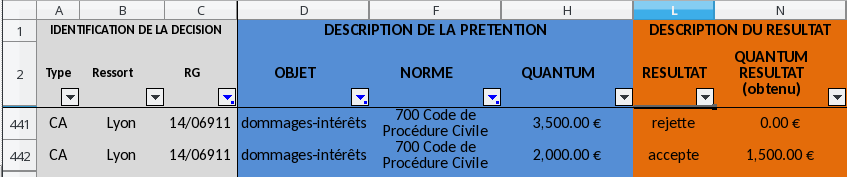
\includegraphics[width=\textwidth]{tab-annotations.png}
		\scriptsize{Les noms des champs sont sur les 2 premières lignes et les demandes sont données en exemple pour la catégorie \textit{dommages-intérêts sur le fondement de l'article 700 du code de procédure civile} (décision 14/06911 de la cour d'appel de Lyon).}
		\caption{Extrait du tableau d'annotations manuelles des demandes.} \label{tab:tab:quanta-annotations}
	\end{table}
\end{enumerate}

%Le résultat d'une phase d'annotation comprend ainsi un tableau des demandes, deux corpus de décisions $D_{c}$ et $D_{\overline{c}}$.

 %Toutes les demandes du corpus $D_{c} \cup D_{\overline{c}}$ annoté manuellement, sont considérées inscrites dans le tableau des annotations manuelles.
 
 La répartition des données d'évaluation est donnée par la Figure \ref{fig:quanta:hist-repartition-docs}. 
 
 \begin{figure}[!htb]
 	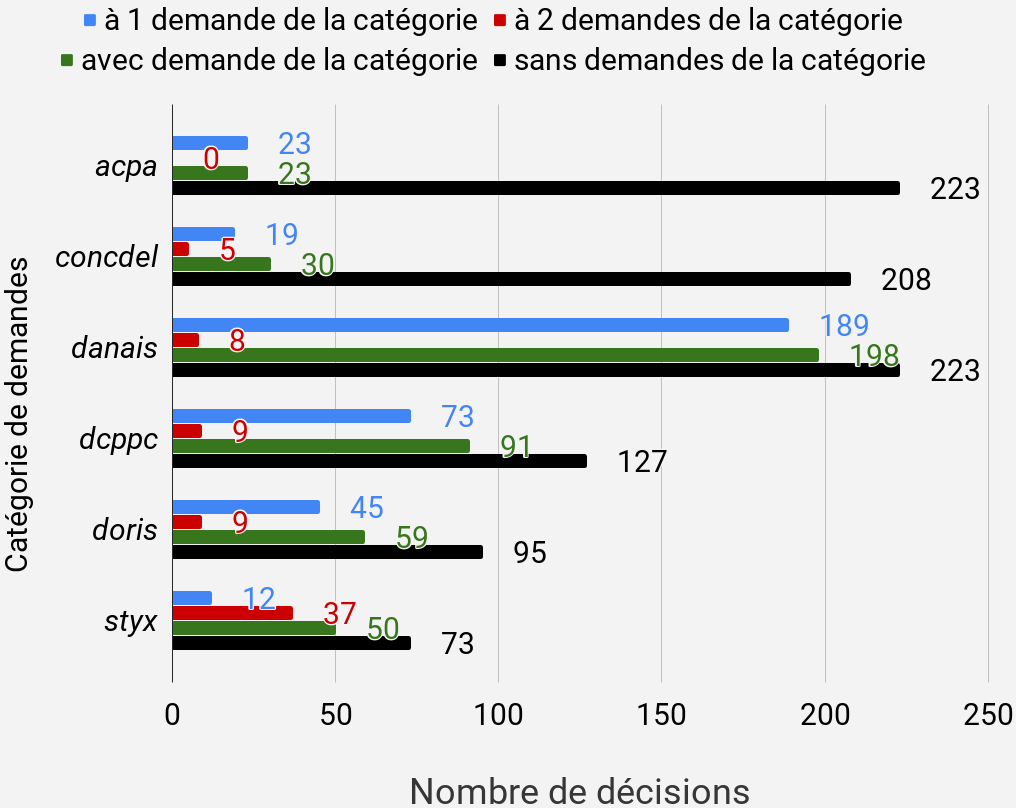
\includegraphics[width=\textwidth]{chartDataset.png}
 	\caption{Répartitions des demandes dans les documents annotées.}\label{fig:quanta:hist-repartition-docs}
 \end{figure}
 
 Il faut aussi noter que bien que l'annotation manuelle des demandes et des résultats soit réalisée dans un tableau (annotation externe au contenu), elle reste une tâche très difficile. Le très faible nombre de documents annotés manuellement en témoigne. Le nombre maximum de documents annotés pour une catégorie est seulement de 198 (barres vertes de \textit{danais}). 

\subsection{Métriques d'évaluation}
\paragraph{Reconnaissance de catégories par classification}

La classification des documents est évaluée en utilisant les métriques précision (P), rappel (R), $F_1$-mesure ($F_1$). %\textcolor{red}{Quelle moyenne: macro / micro?}

\paragraph{Extraction des attributs des paires demande-résultat}
 Nous évaluons les approches proposées sur l'extraction de 3 données: le quantum demandé $q_d$, le sens du résultat $s_r$ et le quantum obtenu $q_r$. Une demande est donc un triplet $(q_d, s_r, q_r)$. Il est possible d'évaluer le système pour un sous-ensemble $x$ de $\lbrace q_d, s_r, q_r \rbrace$ sur les demandes extraites d'un corpus annotées $D$ de test. Nous utilisons les métriques traditionnellement employées en extraction d'information: la précision ($Precision_{c,x,D}$), le rappel ($Rappel_{c,x,D}$), et la F1-mesure ($F1_{c,x,D}$). Ces mesures sont définies à partir des nombres de vrais positifs ($TP$), faux positifs ($FP$) et faux négatifs ($FN$) calculés au niveau d'un document $d$:
\begin{itemize}
\item $TP_{c, x, d}$ est le nombre de demandes extraites de $d$ par le système, qui sont effectivement de la catégorie $c$ (demandes correctes);
\item $FP_{c, x, d}$ est le nombre de demandes extraites de $d$ par le système, mais qui ne sont pas des demandes de $c$ (demandes en trop);
\item $FN_{c, x, d}$ est le nombre de demandes annotées comme étant de $c$ mais qui n'ont pas pu être extraites par le système (demandes manquées).
\end{itemize}

Au niveau d'un corpus d'évaluation $D$, ces métriques sont sommées: 
$TP_{c,x,D} = \sum\limits_{d \in D} TP_{c,x,d}$ \hfill $FP_{c,x,D} = \sum\limits_{d \in D} FP_{c,x,d}$ \hfill $ FN_{c,x,D} = \sum\limits_{d \in D} FN_{c,x,d}$.

Une donnée observée (par exemple \og 3 000 \euro \fg) est bien extraite automatiquement si sa valeur (le nombre $3000$) correspond à celle du quantum annoté dans le tableau. Nous considérons que les unités monétaires, entre les quanta extraits et ceux manuellement annotés, sont identiques.

\subsection{Détection des catégories par classification}
Les implémentations de la bibliothèque Weka \citep{frank2016weka} ont permis d'utiliser plusieurs modèles de classification: le modèle Bayésien naïf (NB), l'arbre de décision C4.5 (implémenté sous l'appelation J48), les k-plus-proches-voisins (KNN), et le SVM. 
 A chaque entraînement, s'exécute une sélection de modèles par validation croisée sur les données d'entraînement. Elle a pour but de sélectionner la métrique locale et la métrique globale appropriée. Les résultats obtenus par 5-\textit{folds} validation croisée sont présentés sur le \tableref{tab:quanta:resultat-detect-cat}. 
 
\begin{table}[!h]
	\scriptsize
	\begin{center}
	\begin{tabular}{l|ccc|ccc|ccc|ccc}
		\hline\noalign{\smallskip}
		& \multicolumn{3}{|c|}{NB} & \multicolumn{3}{|c|}{C4.5} & \multicolumn{3}{|c|}{KNN} & \multicolumn{3}{|c}{SVM} \\ 
		\noalign{\smallskip}
		\hline
		\noalign{\smallskip}
		%Categorie 
		& $P$ & $R$ & $F_1$ & $P$ & $R$ & $F_1$ & $P$ & $R$ & $F_1$ & $P$ & $R$ & $F_1$ \\ 
		\noalign{\smallskip}
		\hline
		\noalign{\smallskip}
		\textit{acpa} & 1.0 & 1.0 & 1.0 & 0.996 & 0.955 & 0.972 & 1.0 & 1.0 & 1.0 & 0.996 & 0.955 & 0.972 \\
		\textit{concdel} & 1.0 & 1.0 & 1.0 & 1.0 & 1.0 & 1.0 & 1.0 & 1.0 & 1.0 & 0.995 & 0.967 & 0.979 \\
		\textit{danais} & 0.988 & 0.989 & 0.988 & 0.996 & 0.995 & 0.995 & 0.995 & 0.995 & 0.995 & 0.993 & 0.993 & 0.993 \\
		\textit{dcppc} & 1.0 & 1.0 & 1.0 & 1.0 & 1.0 & 1.0 & 1.0 & 1.0 & 1.0 & 1.0 & 1.0 & 1.0 \\
		\textit{doris} & 1.0 & 1.0 & 1.0 & 1.0 & 1.0 & 1.0 & 1.0 & 1.0 & 1.0 & 1.0 & 1.0 & 1.0 \\
		\textit{styx} & 1.0 & 1.0 & 1.0 & 0.984 & 0.983 & 0.983 & 1.0 & 1.0 & 1.0 & 1.0 & 1.0 & 1.0 \\
		\hline
	\end{tabular}
\end{center}

$P$= Précision, $R$=Rappel, $F_1$ = $F_1$-mesure
	\caption{Evaluation de la détection de catégories.}\label{tab:quanta:resultat-detect-cat}
\end{table}

D'après les résultats, la détection de catégorie par classification binaire est relativement aisée pour les algorithmes traditionnels qui détectent parfaitement la présence ou non d'une catégorie dans les documents. Par conséquent, pour toute catégorie $c$, les résultats de l'extraction, dans la suite, ne sont discutés que pour les documents de $c$, car, grâce à l'efficacité de la phase de classification, aucun document de $\overline{c}$ ne sera traité par la phase d'extraction.

\subsection{Extraction de données des paires demandes-résultats}
Les scores des termes-clés candidats étant normalisés, si on sélectionne les termes dont les scores sont supérieurs à un seuil fixé, on remarque que chaque métrique d'extraction a un niveau d'efficacité différent entre les catégories de demande (\tableref{tab:quanta:compareGW} avec 0.5 comme seuil fixé). 

\begin{table}[!htb]
	\centering \small
	\begin{tabular}{|c|c|c|c|c|c|c|c|}
		\hline
		& \textit{acpa} & \textit{concdel} & \textit{danais} & \textit{dcppc} & \textit{doris} & \textit{styx} & \textbf{Moyenne} \\ \hline
		$bidf$ & 37.33 & 32.73 & 23.96 & 20.46 & 8.08 & 28.43 & 25.17 \\ \hline
		$\chi^2$ & \textbf{54.55} & 25.88 & 43.97 & 28.35 & 13.11 & 52.73 & 36.43 \\ \hline
		$dbidf$ & 37.58 & 24.63 & 56.25 & \textbf{29.06} & 11.58 & 52.73 & 35.31 \\ \hline
		$\Delta_{DF}$ & \textbf{54.55} & 25.55 & 48.16 & 28.1 & \textbf{19.64} & 52.73 & \textbf{38.12} \\ \hline
		$dsidf$ & 37.58 & 25.25 & \textbf{56.42} & 26.05 & 8.72 & \textbf{53.46} & 34.58 \\ \hline
		$gss$ & \textbf{54.55} & 25.11 & 48.16 & 28.1 & \textbf{19.64} & 52.73 & \textbf{38.05} \\ \hline
		$idf$ & 38.78 & 32.73 & 22.31 & 20.53 & 8.27 & 25.22 & 24.64 \\ \hline
		$ig$ & 4 & 12.4 & 45.21 & 14.99 & 16.74 & 51.13 & 24.08 \\ \hline
		$marascuilo$ & \textbf{54.55} & 23.65 & 43.97 & 26.67 & 17.91 & 52.73 & 36.58 \\ \hline
		$ngl$ & 42.02 & 23.97 & 52.31 & 27.21 & 13.29 & 53.2 & 35.33 \\ \hline
		$pidf$ & 26.19 & \textbf{33.71} & 21.83 & 20.46 & 8.76 & 27.68 & 23.11 \\ \hline
		$rf$ & 41.11 & 33.09 & 55.72 & 28.56 & 14.93 & 51.23 & 37.44 \\ \hline
	\end{tabular}
%\caption{$F1_{c,(q_d, s_r, q_r), D_c}$ moyenne pour une 5-\textit{fold} validation croisée pour chaque métrique de sélection de termes pour un seuil égal à $0.5$}
\caption{Comparaison des pondérations globales suivant la $F_1$-mesure.} \label{tab:quanta:compareGW}
\end{table}

Par conséquent, la métrique et le seuil doivent être bien sélectionnés en fonction de la catégorie de demandes traitée. En choisissant, pour ces hyper-paramètres, les valeurs les plus efficaces pour l'extraction sur la base d'apprentissage, les résultats du \tableref{tab:quanta:resultDetailExtraction} sont observés. Les améliorations sont à noter notamment pour trois catégories. Le score $F_1$ sur l'extraction des triplets $(q_d,s_r, q_r)$ passe de 54.55 au maximum à 58.99 (plus de 4\%) pour \textit{acpa}, de 29.06 à 29.41 pour \textit{dcppc}, de 19.64 à 29.08 (près de 10\%) pour \textit{doris}. Les baisses de performances observées pour les autres catégories est comparativement très faibles (moins de 2\%).
 

\begin{table}[!htb]
\footnotesize
\begin{center}
	\begin{tabular}{l|l|l|llll|llll}
			 \hline
		& & & \multicolumn{4}{c|}{Données d'entraînement} & \multicolumn{4}{c}{Données de test} \\ \hline
		$c$ & Données & $\vert V_c \vert$ & $P$ & $R$ & $F_1$ & \%Docs & $P$ & $R$ & $F_1$ & \%Docs \\ \hline
		\multirow{5}{*}{\textit{acpa}} & $q_d$ & 1 & 86.4 & 56.37 & 68.13 & 56.37 & 68.33 & 54 & 58.99 & 46 \\
		& $q_r$ & 1 & 100 & 65.09 & 78.74 & 65.09 & 93.33 & 63 & 71.43 & 55 \\
		& $s_r$ & 1 & 100 & 65.09 & 78.74 & 65.09 & 93.33 & 63 & 71.43 & 55 \\
		& $(s_r, q_r)$ & 1 & 100 & 65.09 & 78.74 & 65.09 & 93.33 & 63 & 71.43 & 55 \\
		& $(q_d,s_r, q_r)$ & 1 & 86.4 & 56.37 & 68.13 & 56.37 & 68.33 & 54 & 58.99 & 46 \\ \hline
		\multirow{5}{*}{\textit{concdel}} & $q_d$ & 26 & 49.33 & 44.02 & 45.31 & 24.17 & 73.2 & 29.72 & 33.29 & 26.67 \\
		& $q_r$ & 26 & 48.3 & 42.66 & 44.1 & 22.5 & 75.73 & 28.89 & 34.3 & 26.67 \\
		& $s_r$ & 26 & 46.52 & 40.89 & 42.36 & 22.5 & 74.93 & 26.39 & 33.09 & 26.67 \\
		& $(s_r, q_r)$ & 26 & 46.52 & 40.89 & 42.36 & 22.5 & 74.93 & 26.39 & 33.09 & 26.67 \\
		& $(q_d,s_r, q_r)$ & 26 & 42.43 & 37.41 & 38.68 & 20.83 & 68.27 & 23.06 & 28.65 & 23.33 \\ \hline
		\multirow{5}{*}{\textit{danais}} & $q_d$ & 37 & 77.71 & 48.71 & 59.68 & 37.3 & 79.25 & 47.5 & 59 & 37.3 \\
		& $q_r$ & 37 & 77.68 & 48.71 & 59.67 & 37.03 & 77.78 & 46.46 & 57.79 & 36.22 \\
		& $s_r$ & 37 & 77.05 & 48.33 & 59.19 & 37.03 & 77.78 & 46.46 & 57.79 & 36.22 \\
		& $(s_r, q_r)$ & 37 & 77.05 & 48.33 & 59.19 & 37.03 & 77.78 & 46.46 & 57.79 & 36.22 \\
		& $(q_d,s_r, q_r)$ & 37 & 74.45 & 46.65 & 57.16 & 35.81 & 74.41 & 44.38 & 55.23 & 34.59 \\ \hline
		\multirow{5}{*}{\textit{dcppc}} & $q_d$ & 35 & 45.71 & 36.64 & 40.66 & 34.05 & 44.64 & 40.73 & 41.75 & 31.4 \\
		& $q_r$ & 35 & 78.99 & 63.21 & 70.2 & 59.33 & 75.48 & 64.51 & 68.41 & 53.82 \\
		& $s_r$ & 35 & 84.73 & 67.85 & 75.33 & 63.24 & 81.21 & 69.14 & 73.51 & 57.43 \\
		& $(s_r, q_r)$ & 35 & 78.99 & 63.21 & 70.2 & 59.33 & 75.48 & 64.51 & 68.41 & 53.82 \\
		& $(q_d,s_r, q_r)$ & 35 & 34.2 & 27.39 & 30.41 & 28.03 & 31.66 & 28.55 & 29.41 & 25.37 \\ \hline
		\multirow{5}{*}{\textit{doris}} & $q_d$ & 8 & 31.98 & 35.76 & 32.94 & 7.75 & 37.48 & 35.9 & 36.63 & 7.12 \\
		& $q_r$ & 8 & 35.73 & 39.72 & 36.69 & 8.63 & 39.43 & 38.47 & 38.89 & 7.12 \\
		& $s_r$ & 8 & 35.06 & 39.56 & 36.24 & 9.06 & 42.91 & 41.44 & 42.12 & 8.94 \\
		& $(s_r, q_r)$ & 8 & 32.61 & 36.16 & 33.45 & 8.2 & 38.14 & 37.04 & 37.54 & 7.12 \\
		& $(q_d,s_r, q_r)$ & 8 & 24.48 & 27.16 & 25.13 & 5.61 & 29.7 & 28.53 & 29.08 & 7.12 \\ \hline
		\multirow{5}{*}{\textit{styx}} & $q_d$ & 4 & 69.34 & 59.55 & 64.04 & 33.5 & 69.3 & 59.49 & 63.61 & 32 \\
		& $q_r$ & 4 & 75.87 & 65.17 & 70.08 & 31.5 & 74.86 & 64.08 & 68.63 & 28 \\
		& $s_r$ & 4 & 75.87 & 65.17 & 70.08 & 31.5 & 74.86 & 64.08 & 68.63 & 28 \\
		& $(s_r, q_r)$ & 4 & 75.87 & 65.17 & 70.08 & 31.5 & 74.86 & 64.08 & 68.63 & 28 \\
		& $(q_d,s_r, q_r)$ & 4 & 57.61 & 49.44 & 53.19 & 25.5 & 57.24 & 48.36 & 52.08 & 24 \\
			\hline\noalign{\smallskip}
	\end{tabular}
\end{center}

$P$ = Précision, $R$ = Rappel, $F_1$ = $F_1$-mesure
	
\%Docs: proportion de documents dont l'ensemble des données extraites est égale à l'attendu (documents parfaitement traités)

$\vert V_c \vert$: nombre moyen de termes-clés identifiés pour la catégorie $c$
\caption{Résultats détaillés pour l'extraction des données avec sélection automatique de la méthode d'extraction des termes-clés} \label{tab:quanta:resultDetailExtraction}
\end{table}


Ces résultats détaillés font remarquer que les attributs, pris individuellement, présentent d'assez bonnes performances. Cependant, la mise en correspondance des attributs peine toujours à montrer des performances du même rang. On remarque néanmoins que les scores $F_1$ des triplets $(q_d,s_r, q_r)$ sont proches de celles des attributs qui présentent le plus de difficulté. En effet, la sélection préalable permet d'observer sur les données de test, des $F_1$-mesures comprises entre 33.09 \% et 71.43 \% pour les champs $q_d$, $q_r$, et $s_r$, et entre 28.65 \% et 58.99 \% pour les triplets $(q_d,s_r, q_r)$. L'échec de l'extraction des attributs est une des principales causes des faibles performances observées pour la liaison des attributs de paires similaires demande-résultat. Par ailleurs, les données sur le résultat, $s_r$ et $q_r$, sont en générale plus faciles à extraire ($F_1$-mesures entre 42.12 et 71.43 sauf pour \textit{concdel}) que le quantum demandé $q_d$ ($F_1$-mesures entre 41.75 et 63.61 sauf pour \textit{concdel}). %Il est aussi bien de noter qu'une plus grande quantité d'exemples annotés de documents ne semble pas être la garantie d'une meilleure extraction. On remarque en effet que les meilleures performances sont obtenues pour la catégorie disposant du plus faible nombre d'exemples annotés (\textit{acpa}) avec en moyenne un seul terme-clé appris. 
Remarquons aussi que la précision est en général supérieure au rappel; ce qui signifie que la méthode a plus tendance à éviter les valeurs erronées au risque de manquer un nombre important de valeurs correctes. Enfin, la proportion de documents parfaitement traités (dans lesquels toutes les demandes de la catégorie ont été extraites) reste inférieur à la moyenne même pour \textit{acpa} donc le corpus ne comprend que des décisions à une seule demande de cette catégorie. L'unique terme-clef appris ne semble pas suffisant pour identifier toutes les demandes de \textit{acpa} (l'\og article 32-1 \fg{} est un bon indicateur par exemple). La catégorie \textit{doris} enregistre la plus faible valeur pour cette proportion, probablement à cause de la présence dans une même décision de plusieurs demandes pour des raisons très variées du trouble du voisinage (préjudice moral, nuisance sonore, préjudice matériel, préjudice de jouissance, etc.) donc malheureusement les termes-clés ne sont pas tous captés par les méthodes statistiques employées (cf. \tableref{tab:quanta:exemples_termes}). %Dans la suite, divers aspects sont décrits pour expliquer les raisons des limites de l'approche proposée.

\subsection{Analyse des erreurs}

En extraction d'éléments structurés, on retrouve trois types d'erreurs \citep{yang2016jointEntityEvt}: les données manquées (faux négatifs), les données en plus des attendues (faux positifs), et les mauvaises classifications (confusions). La confusion n'est pas discutée ici car les annotations ne sont faites que pour une seule classe. %Les confusions sont évitées dans l'approche proposée par la détection préalable des catégories par classification et l'extraction restreinte à une seule catégorie à la fois. 
Etant donné que la précision est en général supérieure au rappel d'après nos résultats, il est certain que les erreurs sont majoritairement dues aux données manquées comme le confirme le \tableref{tab:quanta:types_erreurs}. 

\begin{table}[!htb]
	\centering\small
	\begin{tabular}{|c|c|c|c|c|}
		\hline
		 & \multicolumn{2}{|c|}{Données d'entraînement} & \multicolumn{2}{|c|}{Données de test} \\ \hline
		& \textbf{\%erreurs FP} & \textbf{\%erreurs FN} & \textbf{\%erreurs FP} & \textbf{\%erreurs FN} \\ \hline
		$q_d$ & 36.90 & 63.10 & 36.52 & 63.48 \\ \hline
		$q_r$ & 32.30 & 67.70 & 34.32 & 65.68 \\ \hline
		$s_r$ & 31.72 & 68.28 & 34.11 & 65.89 \\ \hline
		$(s_r, q_r)$ & 32.32 & 67.68 & 34.39 & 65.61 \\ \hline
		$(q_d,s_r, q_r)$ & 37.77 & 62.23 & 37.72 & 62.28 \\ \hline
	\end{tabular}
\caption{Types et taux d'erreurs (pourcentage en moyenne sur les 6 catégories de demandes)} \label{tab:quanta:types_erreurs}
\end{table}

Trois raisons peuvent expliquer le fait que peu de données attendues soient extraites. 

Premièrement, certaines valeurs d'attributs ne sont pas mentionnées dans les sections Litige et Dispositif utilisées (pourcentages inférieurs à 100 dans les Tableaux \ref{tab:quanta:mentionQd} et \ref{tab:quanta:mentionQr}). Par exemple, les quanta résultat de \textit{doris} sont plus présents dans les Motifs que dans le Dispositif.

\begin{table}[!htb]
	\footnotesize \centering
	\begin{tabular}{|l|l|l|l|l|l|l|}
		\hline
		%\textbf{Catégorie}
		& \textbf{\#$q_d$} & \textbf{\#$q_d\neq NUL$} & \textbf{\# dans doc.} & \textbf{\# dans Litige} & \textbf{\# dans Motifs} & \textbf{\# dans Dispositif} \\ \hline
		\textit{acpa} & 23 & 16 & 16 (100\%) & 16 (100\%) & 9 (56.25\%) & 5 (31.25\%) \\ \hline
		\textit{concdel} & 58 & 56 & 55 (98.21\%) & 55 (98.21\%) & 7 (12.5\%) & 2 (3.57\%) \\ \hline
		\textit{danais} & 208 & 182 & 182 (100\%) & 179(100\%) & 39 (21.43\%) & 23 (12.64\%) \\ \hline
		\textit{dcppc} & 126 & 126 & 122 (96.83\%) & 109 (86.51\%) & 71 (56.35\%) & 65 (51.59\%) \\ \hline
		\textit{doris} & 94 & 83 & 83 (100\%) & 82 (98.80\%) & 21 (25.30)\% & 6 (7.23\%) \\ \hline
		\textit{styx} & 89 & 86 & 86 (100\%) & 86 (100\%) & 12 (13.95\%) & 9 (10.47\%) \\ \hline
	\end{tabular}

	\textit{Les pourcentages ne sont calculés que pour les valeurs non nulles}
	\caption{Taux de quanta demandés ($q_d$) mentionnés dans les documents annotés} \label{tab:quanta:mentionQd}
\end{table}

\begin{table}[!htb]
	\footnotesize \centering
	\begin{tabular}{|l|l|l|l|l|l|l|}
		\hline
		%\textbf{Catégorie}
		& \textbf{\# $q_r$} & \textbf{\# $q_r\neq NUL$} & \textbf{\# dans doc.} & \textbf{\# dans Litige} & \textbf{\# dans Motifs} & \textbf{\# dans Dispositif} \\ \hline
		\textit{acpa} & 23 & 6 & 6 (100\%) & 3 (50\%) & 6 (100\%) & 5 (83.33\%) \\ \hline
		\textit{concdel} & 58 & 8 & 8 (100\%) & 2 (25\%) & 8 (100\%) & 6 (75\%) \\ \hline
		\textit{danais} & 208 & 23 & 23 (100\%) & 15 (65.22\%) & 22 (95.65\%) & 20 (86.96\%) \\ \hline
		\textit{dcppc} & 126 & 76 & 75 (98.68\%) & 55 (72.37\%) & 56 (73.68\%) & 64 (84.21\%) \\ \hline
		\textit{doris} & 94 & 44 & 44 (100\%) & 28 (63.64\%) & 40 (90.91)\% & 24 (54.55\%) \\ \hline
		\textit{styx} & 89 & 30 & 29 (96.67\%) & 16 (53.33\%) & 22 (73.33\%) & 29 (96.67\%) \\ \hline
	\end{tabular}

	\textit{Les pourcentages ne sont calculés que pour les valeurs non nulles}
	\caption{Taux de quanta accordés ($q_r$) mentionnés dans les documents annotés} \label{tab:quanta:mentionQr}
\end{table}

En second, la sélection des termes-clés n'est pas parfaite (Tableau \ref{tab:quanta:exemples_termes}). D'une part, l'ensemble sélectionné ne couvre pas toutes les situations d'expression de la catégorie (par exemple, pour la catégorie \textit{styx}, le terme \og frais irrépétibles\fg{} est souvent utilisé à la place de \og article 700 du code de procédure civile\fg{}, mais dans très peu d'exemples annotés). D'autre part, certains termes sont trop spécifiques à la base d'apprentissage (par exemple, pour la catégorie \textit{concdel}, des sommes d'argent et autres termes comme \og condamner in solidum les sociétés \fg{} apparaissent dans la liste).

\begin{table}[!htb]
		\centering\footnotesize
	\begin{tabular}{|c|p{0.8\textwidth}|}
		\hline
		{Catégorie} & \multicolumn{1}{c|}{Termes-clés appris} \\ \hline
		\textit{acpa} & amende civile  \\ \hline
		\textit{concdel} & titre de la concurrence déloyale, somme de 15000euros à titre, réparation de son préjudice financier, payer la somme de 15000euros, condamner in solidum les sociétés, agissements constitutifs de concurrence déloyale \\ \hline
		\textit{danais} & dommages et intérêts pour procédure, 32-1 du code de procédure, intérêts pour procédure abusive, titre de dommages-intérêts pour procédure, intérêts pour procédure, article 32-1 du code, dommages-intérêts pour procédure abusive \\ \hline
		\textit{dcppc} & admet la créance déclarée, admet la créance, passif de la procédure collective, passif de la procédure, hauteur de la somme, créance déclarée, titre chirographaire, admission de la créance, rejette la créance, \\ \hline
		\textit{doris} & préjudices, abusive, condamner solidairement, solidairement, réparation du préjudice, réparation, titre de dommages et intérêts, dommages, titre de dommages, dommages et intérêts, titre de dommages-intérêts, payer aux époux, jouissance \\ \hline
		\textit{styx} & 700 du code de procédure, article 700 du code, 700 du code, article 700, 700  \\ \hline
	\end{tabular}

Les termes candidats sont des $n$-grammes de taille variant d'1 à 5 mots consécutifs
\caption{Premiers termes sélectionnés lors de la première itération de la validation croisée} \label{tab:quanta:exemples_termes}
\end{table}

Enfin, les expérimentations ont été réalisées sur des décisions d'appel mais les énoncés de demande et résultat renvoyant aux décisions de jugements antérieurs ne sont pas encore traités. Ces références aux décisions antérieures représentent une part importante des demandes des décisions d'appel. Il est donc nécessaire de les intégrer explicitement dans le processus d'extraction, pour compléter les données extraites.

\section{Conclusion}
\label{sec:quanta:conclusion}
Ce chapitre décrit le problème d'extraction de données pertinentes relatives aux paires demande-résultat mentionnées dans les décisions de justice. Les divers défis relatifs à la tâche y sont discutés en remarquant des analogies avec d'autres tâches classiques de la fouille de données textuelles. Il a été démontré la solvabilité du problème par la proposition et l'expérimentation d'une approche d'extraction basée sur la terminologie de la catégorie des demandes à extraire et autres connaissances du domaine judiciaire telles que les motifs d'énoncés de demandes et de résultats, ainsi que leur position conventionnelle dans les documents. Les expérimentations démontrent que l'approche permet d'extraire plus ou moins bien des demandes selon la catégorie traitée. Même si nos résultats ont été obtenus à partir de terminologies apprises, une liste de termes fournis par les experts pourrait être plus précise et mettrait à l'abris des biais liés aux échantillons d'apprentissage. A cause de la forte dépendance aux subtilités de rédaction des décisions judiciaires, la méthode proposée rencontre des limites qui ne peuvent être surmontées qu'en la rendant beaucoup plus complexe qu'elle ne l'est déjà. Des approches d'apprentissage automatique sont recommandées comme perspectives. Elles devront être capables d'apprendre l'emplacement des données à extraire de manière semi-supervisée à l'aide de faibles quantités de longs documents annotés.
